\chapter{TINJAUAN PUSTAKA}

\section{PT Bisma Jaya}

\noindent PT Bisma Jaya merupakan perusahaan yang bergerak di industri transportasi angkutan laut yang berbasis di Balikpapan, Kalimantan Timur. Sejak tahun 2011, perusahaan telah menyediakan berbagai jenis kapal untuk kebutuhan transportasi industri. Dalam menjalankan tugasnya PT Bisma Jaya memiliki struktur organisasi seperti pada Gambar 2.1.

\begin{figure}[!h]
    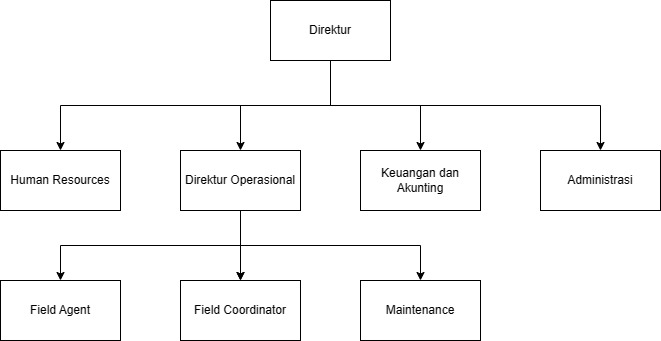
\includegraphics[width=1\linewidth, center]{images/tinjauan-pustaka/fig-org-structure.jpg}
    \caption{Struktur Organisasi PT Bisma Jaya}
    \label{fig:org-structure}
\end{figure}

Gambar 2.1 memberikan gambaran struktur organisasi dari PT Bisma Jaya yang dipimpin oleh Direktur yang membawahi \textit{Human Resource}, Direktur Operasional, Keuangan dan Akunting, dan Administrasi. Direktur Operasional membawahi beberapa bagian seperti \textit{Field Agent}, \textit{Field Coordinator}, dan \textit{Maintenance}. Dalam penelitian ini, peneliti akan lebih banyak berkomunikasi dengan Direktur Operasional mengenai hal teknis maupun non teknis selama pengembangan sistem monitoring. 

\section{\textit{Internet of Things}}

\noindent \textit{Internet of Things (IoT)} merujuk pada keterhubungan antara obyek, perangkat, mesin satu dengan lainnya dan internet mengizinkan mereka untuk mengumpulkan dan menukar data \parencite{inproc:gazis}. Secara arsitektur IoT dapat dibagi menjadi 4 lapisan utama: \textit{sensing layer}, \textit{network layer}, \textit{data processing layer}, dan \textit{application layer} \parencite{article:sikder}. Detailnya dapat dilihat pada Gambar 2.2

\begin{figure}[ht]
    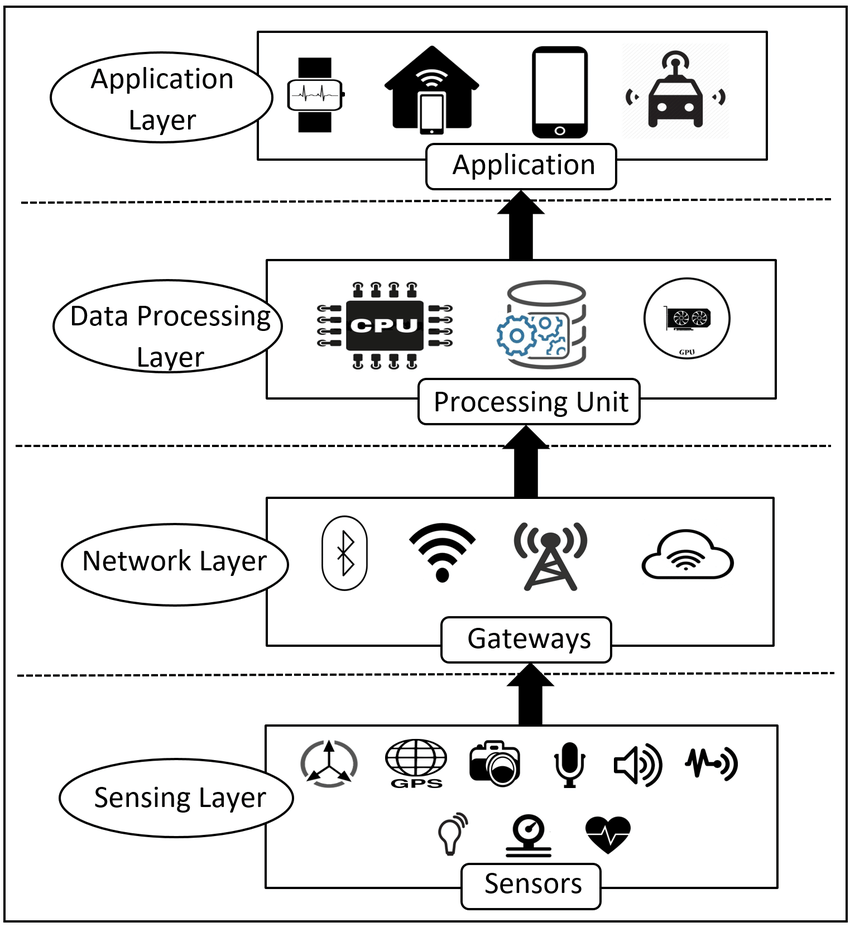
\includegraphics[width=0.6\linewidth, center]{images/tinjauan-pustaka/fig-iot-architecture.png}
    \caption{Lapisan dan Komponen Arsitektur IoT \parencite{article:sikder}}
    \label{fig:iot-architecture}
\end{figure}

\noindent Berikut gambaran umum pada setiap lapisan:
\begin{enumerate}
    \item \textbf{\textit{Sensing Layer}}
    
    Lapisan ini bertanggung jawab untuk memanfaatkan berbagai sensor dan perangkat untuk mengumpulkan data. Sensor seringkali memberikan data berupa angka mentah seperti tegangan. Oleh karena itu, perangkat IoT dapat memprosesnya terlebih dahulu sebelum dikirim ke server - disebut juga dengan \textit{edge-computing} - atau langsung meneruskan data tersebut ke lapisan jaringan untuk diproses di server.
    

    \item \textbf{\textit{Network Layer}}
        
    Lapisan ini bertugas mengirimkan data yang diperoleh sensor ke lapisan pemrosesan data untuk diolah. Lapisan ini juga bertugas mengawasi bagaimana perangkat jaringan IoT berkomunikasi satu sama lain. Untuk menjaga keamanan komunikasi, digunakan token autentikasi setiap adanya pengiriman data ke \textit{server}.

    \item \textbf{\textit{Data Processing Layer}}
    
    Pemrosesan dan analisis data sensor berada di bawah lingkup lapisan ini. Selain itu, ia bertugas mengelola dan menyimpan data. Lapisan pemrosesan data sangat penting untuk menghasilkan \textit{insight} berharga dan mengambil tindakan yang sesuai berdasarkan data yang dikumpulkan.
    
    \item \textbf{\textit{Application Layer}}
    
    Dengan menggunakan data yang dikumpulkan dan diproses, lapisan ini bertanggung jawab untuk memberikan \textit{actionable insight} kepada pengguna akhir. Ini bertugas memastikan kerahasiaan dan keamanan data yang diproses dan dianalisis dan merupakan lapisan teratas dalam arsitektur IoT. 

\end{enumerate}

\section{Raspberry Pi}

\noindent Raspberry Pi merupakan \textit{single-board computer} (SBC) yang telah mendapatkan perhatian dan popularitas yang signifikan dalam beberapa tahun terakhir. Teknologi inovatif ini memungkinkan berbagai penerapan dan sekarang penting dalam bidang ilmu dan teknik komputer \parencite{article:johnston}. Raspberry Pi adalah pilihan yang bagus untuk aplikasi \textit{Internet of Things} (IoT) karena portabilitasnya, paralelismenya, keterjangkauannya, dan konsumsi dayanya yang rendah \parencite{article:hosny}. Hal yang membuat Raspberry Pi dapat diandalkan sebagai perangkat IoT adalah adanya 40 pin GPIO yang memungkinkan ia dihubungkan ke beragam sensor dengan berbagai \textit{interface}. Raspberry Pi serta informasi GPIO dapat dilihat pada Gambar 2.3.

\begin{figure}[!h]
    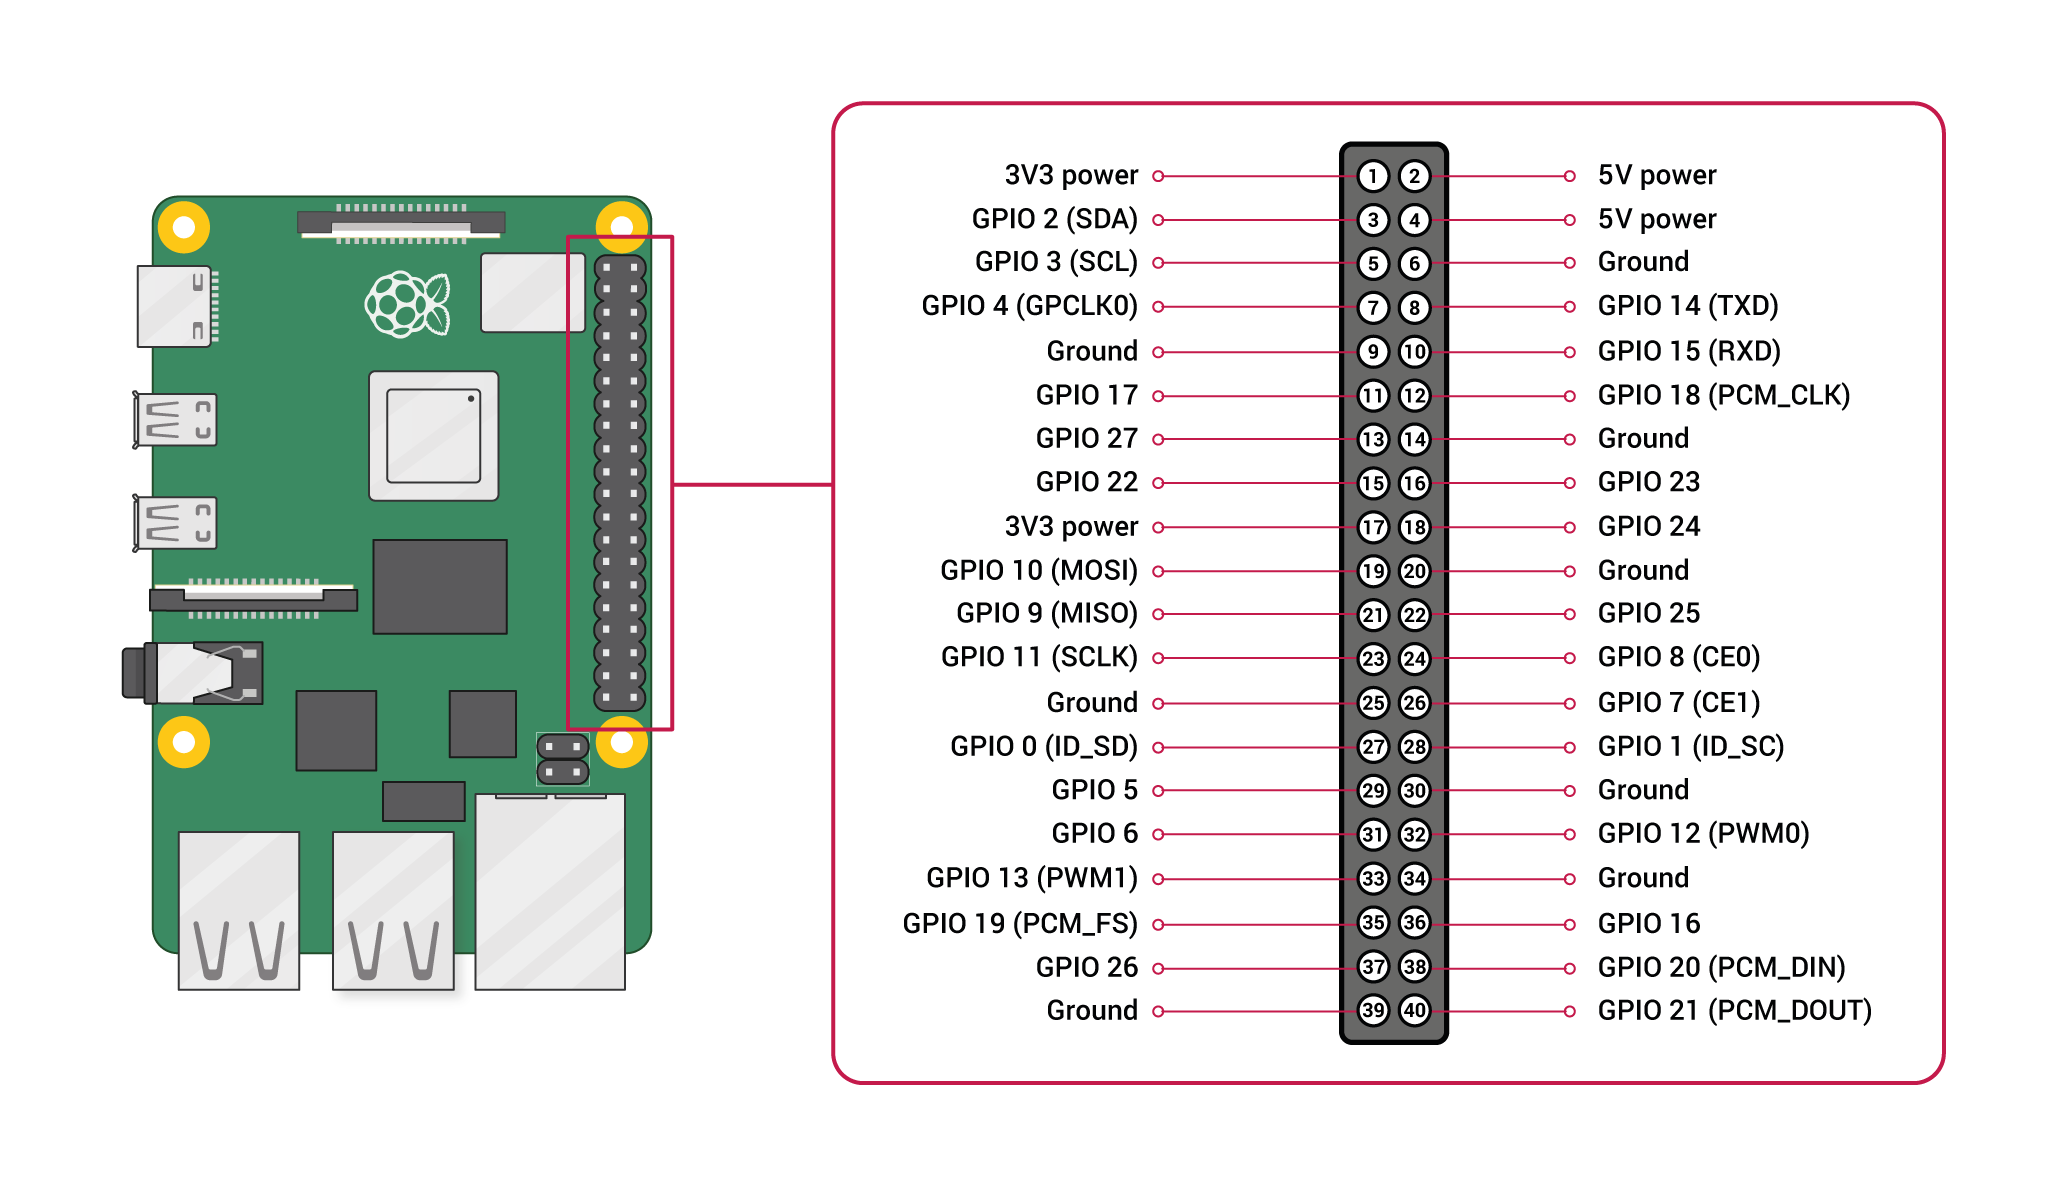
\includegraphics[width=0.9\linewidth, center]{images/tinjauan-pustaka/fig-raspy.png}
    \caption{Raspberry Pi dan 40 pin GPIO}
    \label{fig:raspy}
\end{figure}

Setiap pin GPIO dapat digunakan sebagai pin input maupun output, dan dapat digunakan untuk berbagai kebutuhan. Terdapat pin 5v dan 3.3v yang berjumlah masing-masing 2, juga beberapa pin \textit{ground} yang tidak dapat dikonfigurasi. Sisanya merupakan pin \textit{general purpose} 3.3v, yang berarti  output diatur ke 3.3v dan input toleran dengan nilai 3.3v. Pin output dapat diatur ke \textit{high} (3.3v) dan \textit{low} (0v). Begitu juga dengan pin input, dapat membaca \textit{high} (3.3v) dan \textit{low} (0v). Selain itu, pin GPIO juga dapat digunakan untuk kebutuhan yang memerlukan jenis pin yang spesifik seperti \textit{PWM (pulse-width modulation)} untuk membuat sinyal analog; \textit{SPI (serial peripheral interface)} untuk transfer data antar Raspberry Pi dengan perangkat periferal; \textit{I2C (inter-integrated circuit)} untuk komunikasi dengan berbagai jenis sensor; dan Serial untuk pembacaan data serial.

\section{NextJS}

\noindent NextJS merupakan \textit{framework} JavaScript yang menjadi standar pengembangan web modern berbasis JavaScript. JavaScript sendiri merupakan bahasa pemrograman yang sering digunakan khususnya pada pemrograman web. Menurut \textcite{article:tomasdottir}, JavaScript dikenal dengan sifatnya yang dinamis, yang mencakup fitur-fitur seperti \textit{dynamic typing}, \textit{dynamic file loading}, \textit{first-class functions}, dan \textit{property access}. JavaScript juga merupakan bahasa yang \textit{dynamically typed} meskipun sistem \textit{static type} seperti TypeScript dan Flow telah dibuat untuk itu,  \parencite{article:gao}. JavaScript adalah pilihan yang bagus untuk pembuatan aplikasi dengan tampilan data yang dinamis.

\section{Django}

\noindent Django merupakan \textit{framework} Python dalam pengembangan web. Pada penelitian ini Django digunakan sebagai perantara bagi modul IoT dan database berinteraksi melalui API. Python adalah bahasa pemrograman populer yang digunakan secara luas di berbagai bidang. Ia terkenal dengan syntaxnya yang singkat dan sederhana, sehingga cocok untuk otomatisasi proses dan pengintegrasian aplikasi \parencite{article:buhler}. Popularitas Python dapat dikaitkan dengan kemampuan beradaptasi dan ketersediaan berbagai \textit{library} dan \textit{framework} yang mempercepat dan menyederhanakan pengembangan \parencite{article:malloy}.

\section{MySQL}

\noindent MySQL adalah sistem manajemen \textit{database open-source} yang umum digunakan sebagai penghubung perangkat lunak dengan \textit{database} server. MySQL dapat secara efektif mengelola banyak pengguna secara bersamaan dan data dalam jumlah besar \parencite{article:gomez}. Oleh karenanya, database ini cocok digunakan untuk menyimpan log data yang akan diterima dari sensor.

\section{\textit{Entity Relationship Diagram}}

\noindent \textit{Entity relationship diagram} basis data direpresentasikan secara visual dalam diagram hubungan entitas (ERD). Dengan menggunakan metode \textit{top-down}, ini mewakili hubungan antara entitas dan atributnya dan mengatur data berdasarkan informasi semantik \parencite{article:chen}. Untuk memberikan representasi yang jelas dan ringkas tentang struktur dan hubungan dalam database, ERD sering digunakan dalam desain dan pemodelan database \parencite{article:supriyadi}.

\section{Metode Perhitungan Bahan Bakar}

\noindent Dokumen Fuel Consumption Rate Verification (FCRV) merupakan dokumen yang berisi informasi kategori operasi berdasarkan rentang kecepatan tertentu. Ini akan digunakan awak kapal ketika hendak melaporkan jumlah konsumsi bahan bakar berdasarkan jumlah running hour pada rentang angka kecepatan yang telah ditentukan. Berikut contoh isi dari Dokumen FCRV.

\begin{table}[!h]
    \centering
     \begin{tabular}{c c c c} 
        \toprule
        Operation Category & 
        Max Fuel Used (L) & 
        RPM & 
        Average Speed (knot) \\ [0.5ex] 
        \midrule
        Full Speed          & 28    & 1100      & 5 \\  
        Economical Speed    & 18    & 900-1000  & 4 \\  
        Slow Speed/Maneuver & 11    & 700-800   & 3 \\  
        Idle Speed          & 6     & 600       & 0 \\  
        Standby (M/E Off)   & 0     & 0         & 0 \\ [1ex] 
        \bottomrule
     \end{tabular}
     \caption{Fuel Consumption Rate Verification}
     \label{tab:fcrv}
\end{table}

Pada tabel diatas, terdapat 4 kategori operasi yakni Full Speed, Economical Speed, Slow Speed/Manuever, dan Idle Speed. Full Speed adalah kondisi kecepatan mesin tertinggi yang hanya digunakan di laut lepas, nilai maksimum konsumsi bahan bakar (FCR) dalam 1 jam mencapai 28L. Lalu, terdapat Economical Speed. Ini merupakan kategori kecepatan tertinggi kedua dan yang paling sering digunakan ketika menyusuri sungai. Kategori ini memiliki rentang RPM 900-1000 dengan nilai FCR 18L dalam 1 jam. Selanjutnya terdapat Slow Speed, dimana kecepatan ini digunakan untuk mengatur posisi kapal di pelabuhan. Kategori ini memiliki rentang RPM 700-800 dengan nilai FCR 11L dalam 1 jam. Terakhir, Idle Speed dimana kapal dalam kondisi tidak bergera namun mesin menyala. Rentang RPM pada kategori ini adalah 700 kebawah dan hanya memakan bahan bakar 6L dalam 1 jam.

Pada praktiknya, awak kapal hanya mengisi nilai running hour dari masing-masing kategori untuk mendapatan nilai konsumsi bahan bakar. Nilai running hour ini didapatkan berdasarkan estimasi mengikuti jurnal aktivitas/pergerakan kapal. Contoh pengisian tabelnya adalah sebagai berikut.


\begin{table}[!h]
    \centering
     \begin{tabular}{c c c} 
        \toprule
        Running Hour & 
        Operation Category & 
        Fuel Consumption (L) \\ [0.5ex] 
        \midrule
        01:00   & Full Speed            & 28    \\  
        02:30   & Economical Speed      & 45    \\  
        00:30   & Slow Speed/Manuever   & 5.5   \\  
        00:10   & Idle Speed            & 1     \\ [1ex] 
        \bottomrule
     \end{tabular}
     \caption{Contoh Laporan Penggunaan Bahan Bakar}
     \label{tab:fc-report-example}
\end{table}

\section{Perbandingan SDLC}

\noindent Berikut adalah perbandingan dari metodologi \textit{Extreme Programming} dengan salah satu metode sequential, yaitu Waterfall dan metode Agile lainnya, yaitu Scrum menurut \textcite{inproc:fahrurrozi} dan \textcite{article:suryantara}. 

\begin{longtable}[!h]
        {
            p{0.19\textwidth}
            p{0.27\textwidth}
            p{0.27\textwidth}
            p{0.27\textwidth}
        }
        
        \toprule
        Tahapan dalam pengembangan & \textit{Extreme Programming} & Waterfall & Scrum \\ [0.5ex] 
        \midrule
        \textit{Planning} 
        & 
        Pada tahap ini dilakukan pengumpulan kebutuhan sistem dan menjadikannya dalam bentuk user story dan diurutkan berdasarkan tingkat kesulitannya. 
         
        & 
        Tahap ini merupakan langkah awal dimana kebutuhan proyek dikumpulkan dan dianalisis.  
        
        & 
        Tahap ini dibagi menjadi 2 bagian: Sprint \textit{Planning} dan Release \textit{Planning}. Sprint \textit{Planning} dilakukan setiap awal sprint dan Release \textit{Planning} dilakukan setiap awal rilis. 
         
        \\
        \midrule

        \textit{Analysis} 
        & 
        Developer kemudian memutuskan user story apa saja yang akan dikerjakan pada iterasi mendatang 
        & 
        Pada Tahap ini kebutuhan yang dikumpulkan akan dipecahkan menjadi potongan yang dapat dikelola
        
        & 
        Analisis terjadi saat Sprint \textit{Planning}, dimana tim akan memilih perkerjaan yang akan mereka selesaikan di sprint tersebut
        
        \\ 
        \midrule

        \textit{Design} 
        & 
        Tim bekerja dalam iterasi singkat untuk menghasilkan software yang berfungsi, dan desainnya berkembang seiring kemajuan proyek
        & 
        Tahap desain melibatkan pembuatan rencana rinci untuk software berdasarkan persyaratan yang dikumpulkan dalam fase perencanaan dan analisis. 
        & 
        Perancangan terjadi selama Sprint \textit{Planning}, dimana tim memilih pekerjaan yang akan mereka selesaikan selama sprint 
        
        \\ 
        \textit{Implementation} 
        & 
        Developer bekerja dalam waktu singkat untuk menghasilkan software yang berfungsi, dan implementasinya berkembang seiring kemajuan proyek
        & 
        Tahap implementasi melibatkan koding software berdasarkan rencana rinci yang dibuat pada fase desain 
        & 
        Implementasi terjadi selama sprint, dimana tim menyelesaikan pekerjaan yang mereka pilih selama Sprint \textit{Planning} 
        
        \\ 
        \midrule

        \textit{Support \& Security} 
        & 
        Support dan security adalah proses yang berlangsung sepanjang proyek. Tim bekerja dalam waktu singkat untuk menghasilkan software yang berfungsi, dan perangkat lunak tersebut terus diperbarui dan dipelihara
        & 
        Tahap support dan security terjadi setelah software dikirimkan. Tahap ini melibatkan pemeliharaan dan pembaruan perangkat lunak untuk memastikannya terus memenuhi kebutuhan pengguna 
        & 
        Support dan security terjadi setelah perangkat lunak dikirimkan. Fase ini melibatkan pemeliharaan dan pembaruan perangkat lunak untuk memastikannya terus memenuhi kebutuhan pengguna 
        \\ [1ex] 

        \bottomrule
    \caption{Perbandingan metodologi SDLC}
    \label{tab:sdlc-comparison}
\end{longtable}

\section{\textit{Extreme Programming} (XP)}

\noindent \textit{Extreme Programming} (XP) adalah pendekatan \textit{agile software development} yang memberikan penekanan pada kerja sama, pengembangan iteratif dan berulang, serta kemampuan beradaptasi terhadap perubahan kebutuhan. XP merupakan metodologi sederhana yang dibuat untuk tim pengembang kecil yang bertujuan untuk meningkatkan kualitas dan produktivitas perangkat lunak \parencite{article:matharu}. Kesulitan yang ditimbulkan oleh siklus pengembangan yang panjang dalam praktik pengembangan perangkat lunak konvensional menyebabkan terciptanya XP \parencite{article:rao}.

Ada berbagai prinsip dasar yang mendefinisikan XP. \textit{Continuous planning}, yang memerlukan komunikasi dan kolaborasi rutin antara pengembang dan pemangku kepentingan untuk memastikan bahwa tujuan dan persyaratan proyek dipahami dan dipenuhi \parencite{article:matharu}. Siklus hidup pada metode \textit{Extreme Programming} meliputi \textit{Exploration Phase}, \textit{Planning Phase}, \textit{Iteration to Release Phase}, \textit{Productionizing Phase}, \textit{Maintenance Phase}, dan \textit{Death Phase}. Lebih lengkapnya dapat dilihat pada gambar berikut.

\begin{figure}[ht]
    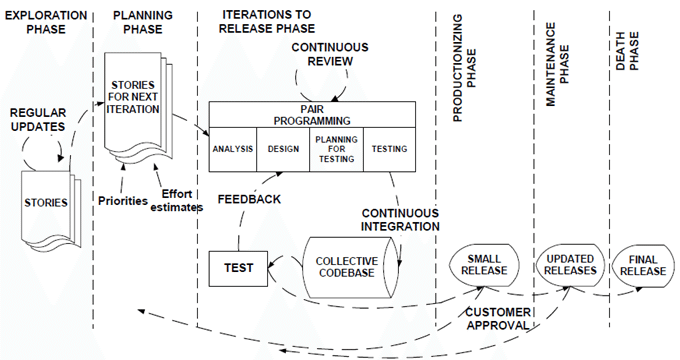
\includegraphics[width=1\linewidth, center]{images/tinjauan-pustaka/fig-xp-lifecycle.png}
    \caption{Siklus Hidup Metode \textit{Extreme Programming} \parencite{article:anwer}}
    \label{fig:xp-lifecycle}
\end{figure}

Berikut penjalasan detail untuk setiap fase:
\begin{enumerate}
    \item \textbf{Exploration Phase:}
    Pada fase ini, dihasilkan user story yang dibuat berdasarkan hasil pengambilan data baik dari observasi, interview, dan dialog dengan mitra. User story ini dapat bertambah seiring waktu mengikuti kebutuhan mitra.

    \item \textbf{Planning Phase:}
    Selanjutnya, user story yang sebelumnya dibuat akan dikumpulkan dan diprioritaskan berdasarkan perhitungan poin story. Ini akan membantu kita dalam menentukan user story mana yang akan dikerjakan pada iterasi berikutnya.
    
    \item \textbf{Iteration to Release Phase:}
    Tahap iterasi merupakan tahap dimana pengembang akan mengimplementasi sistem berdasarkan user story yang ditentukan. Pertama, dilakukan tahap analisis untuk mengonversi kebutuhan mitra menjadi user flow untuk desain tampilan dan algoritma untuk logika sistem. Lalu, dilakukan desain tampilan sesuai dengan user flow yang dihasilkan dan dilakukan perencanaan untuk pengujian. Terakhir, dilakukan pengujian oleh pengembang sebelum kode diunggah ke repositori. Proses programming dilakukan secara parallel dari tahap analisis hingga pengujian. Setelah sistem berhasil melewati unit test dan integration test, sistem akan diuji oleh mitra dan hanya dapat lanjut ke tahap berikutnya setelah mendapatkan persetujuan.
    
    \item \textbf{Productionizing Phase:}
    Sistem yang telah diunggah di repositori akan diluncurkan di server dengan mode development. Ini memungkinkan mitra untuk melakukan pengujian fitur yang masih dalam proses persetujuan serta memberikan umpan balik secara berkala. 
    
    \item \textbf{Maintenance Phase:}
    Iterasi yang mendapatkan persetujuan selanjutnya akan diluncurkan pada tahap ini. Dapat dikatakan sistem yang terdapat pada tahap ini merupakan gambaran terakhir dari sistem secara keseluruhan.
    
    \item \textbf{Death Phase:}
    Ini merupakan tahap terakhir dimana sistem akan diluncurkan secara penuh di server dengan mode production.
\end{enumerate}

Melihat dari tantangan industri mitra yang dinamis serta perlunya kolaborasi yang kuat dari berbagai lintas disiplin ilmu untuk mewujudkan Sistem Monitoring berbasis IoT ini, diputuskanlah metode Extreme Programming sebagai metodologi pengembangan perangkat lunak yang menekankan pada komunikasi dan kolaborasi serta sifatnya yang agile memungkinkan pengembang untuk menjawab berbagai tantangan industri tanpa interupsi selama proses pengembangan sistem.

\section{Penelitian Terdahulu}

\noindent Berikut rangkuman hasil penelitian terdahulu yang memiliki keterkaitan dengan penelitian yang dilakukan.

\begin{longtable}[!h]
        {
            p{0.05\textwidth}
            p{0.3\textwidth}
            p{0.65\textwidth}
        } 
        \toprule
        No & 
        Nama Peneliti dan Tahun & 
        Penelitian yang dilakukan \\ [0.5ex] 
        \midrule
        
        1
        & \textcite{inproc:abdulmalek}
        &
        \textbf{Judul:}
        \textit{IoT-Based Healthcare-Monitoring System towards Improving Quality of Life: A Review}

        \textbf{Permasalahan:}
        Kelemahan utama dari layanan kesehatan adalah hanya tersedia di rumah sakit, sehingga tidak memadai dan terkadang tidak mampu memenuhi kebutuhan lansia dan penyandang disabilitas. Pemantauan status kesehatan lansia secara real-time adalah masalah yang diselesaikan secara efektif dan praktis oleh \textit{Internet of Things} (IoT) dengan penggunaan data sensor dan telekomunikasi.

        \textbf{Hasil:}
        Sistem kesehatan berbasis IoT memfasilitasi hidup orang dalam banyak cara.
        
        \begin{enumerate}
            \item \textbf{Remote healthcare:}
            Daripada pasien mendatangi layanan kesehatan, solusi nirkabel berbasis IoT menghadirkan layanan kesehatan kepada pasien. Sensor berbasis IoT digunakan untuk mengumpulkan data dengan aman, yang kemudian diproses oleh algoritma kecil dan dibagikan kepada penyedia layanan kesehatan untuk mendapatkan rekomendasi yang tepat.

            \item \textbf{Realtime monitoring:}
            Sensor pemantauan berbasis IoT mengumpulkan serangkaian data psikologis. Penyimpanan data dikelola melalui analisis dan \textit{gateway} berbasis \textit{cloud}.
    
    
            \item \textbf{Preventive care:}
            Data sensor digunakan oleh sistem layanan kesehatan IoT untuk memberi tahu anggota keluarga dan membantu deteksi dini keadaan darurat. \textit{Internet of Things} memungkinkan machine learning untuk deteksi anomali dini dan pelacakan tren kesehatan.
        \end{enumerate}
        
        \\

        2
        & \textcite{article:anh}
        & 
        \textbf{Judul:} 
        \textit{Development and Implementation of a low-cost IoT System for Small Farm Households}

        \textbf{Permasalahan:}
        Pertanian kecil memiliki peran yang yang penting untuk produksi agrikultural terutama pada negara kurang berkembang maupun berkembang. Berbeda dengan pertanian skala besar yang berinvestasi pada teknologi mutakhir untuk memastikan kualitas hasil panen yang maksimal, teknologi pada pertanian kecil masih sangat terbatas. 

        \textbf{Hasil:}
        Sistem IoT diusulkan untuk dapat membantu petani kecil meningkatkan kualitas produk pertanian sekaligus mengurangi biaya produksi dan mencegah pemborosan air irigasi dan pupuk. Agrikultur sangat bergantung pada cuaca dan iklim, seperti temperatur dan kadar air tanah. Dalam penelitian, sistem melakukan monitoring pada temperatur, kelembapan, intensitas cahaya, dan kadar air tanah. Parameter tersebut digunakan sebagai acuan dalam mengatur pompa embun, pompa irigasi, jendela ventilasi, kipas ventilasi, dan grow light. 

        \\ 
        
        3
        & \textcite{inproc:hizbullah} 
        &   
        \textbf{Judul:} \textit{Internet of Things} for Smart Transportation in North Moluccas Province

        \textbf{Permasalahan:} Perlunya transportasi yang lebih aman dan penyediaan layanan keselamatan selama keadaan darurat di wilayah Provinsi Maluku Utara.

        \textbf{Hasil:} Diterapkan otomasi pada sistem navigasi yang dapat membantu meningkatkan akurasi dan keandalan navigasi perahu agar mengurangi risiko kecelakaan. Peneliti juga menerapkan sistem monitoring yang dapat menyediakan data secara real-time terhadap kondisi perahu untuk kebutuhan maintenance dan deteksi lebih awal isu yang mungkin akan terjadi.
        
        \\ 
        \midrule

        4
        & \textcite{article:maswadi} 
        &   
        \textbf{Judul:} \textit{Systematic Literature Review of Smart Home Monitoring Technologies Based on IoT for the Elderly}

        \textbf{Permasalahan:} Dengan seiring bertambahnya populasi lansia berumur 65 keatas di negara-negara seperti Amerika, Jerman, Perancis, Itali, dan Jepang terdapat kemungkinan mereka akan beban yang bertambah pada kesehatan dan layanan sosial. Diperlukan teknologi yang dapat memberikan lingkungan hidup yang kondusif bagi para lansia.

        \textbf{Hasil:} Penerapan teknologi sistem smart home pada lansia telah secara signifikan meningkatkan kualitas hidup diantara para lansia. Beberapa teknologi yang dilaporkan telah menyelamatkan hidup para lansia di situasi darurat. 
        
        \\ 

        5
        & \textcite{article:song} 
        &   
        \textbf{Judul:} \textit{Internet of Maritime Things Platform for Remote Marine Water Quality Monitoring}

        \textbf{Permasalahan:} Penerapan sistem monitoring kualitas air di laut memerlukan dukungan komunikasi jarak jauh dan berkecepatan tinggi yang stabil.

        \textbf{Hasil:} Dalam penelitian ini, dikembangkan sebuah platform IoT Maritim yang mendukung komunikasi jarak jauh dan berkecepatan tinggi untuk pemantauan kualitas air laut jarak jauh dan online. Perangkat ditempatkan di atas permukaan air laut dan gerbang untuk pengiriman data ditempatkan darat. Untuk merealisasi komunikasi jarak jauh dan berkecapatan tinggi antara perangkat dengan control center di darat, dikembangkan sistem penyesuaian sinar otomatis (automatic beam adjustment system) untuk antena pengarah sehingga dapat mendukung komunikasi jarak jauh dan berkecepatan tinggi dengan secara otomatis mengatur derajat sinar agar selalu mengarah ke gateway di darat. Metode ini terbukti memberikan performa komunikasi dua kali lipat dibandingkan koneksi nirkabel (LTE di laut) yang ada.
        
        \\
        \bottomrule
     \caption{Penelitian terdahulu mengenai \textit{Internet of Things} (IoT)}
     \label{tab:prev-research}
\end{longtable}